


\documentclass[10pt]{article}
\label{articlepackage}

%\usepackage{tgbonum}
\usepackage{soul}
%\usepackage{hyperref}
\usepackage{multicol}

\usepackage{setspace}
\usepackage{slashed}
%\doublespacing

\usepackage[T1]{fontenc}
\usepackage{ifthen}
\usepackage{mathrsfs}


\usepackage{bm}
\usepackage{bibentry}
\usepackage{subcaption}
\usepackage{wrapfig}
\usepackage{amsmath}
\numberwithin{equation}{section}
\numberwithin{figure}{section}
\numberwithin{table}{section}
\numberwithin{footnote}{section}
\usepackage{mathtools}
\usepackage[inline]{enumitem}
\usepackage{booktabs}
%\usepackage[usenames,dvipsnames,pdftex]{xcolor}
\usepackage{tikz}
\usetikzlibrary{backgrounds,shapes,arrows,positioning,calc,snakes,fit}
\usepgflibrary{decorations.markings}
\usepackage{framed}

% \setcounter{section}{-1}

\usepackage{graphicx} % standard package
\usepackage{todonotes} % standard package
\usepackage{amsmath} % standard package
\DeclareMathOperator{\sech}{sech}
\newcommand*\diff{\mathop{}\!\mathrm{d}}
\newcommand{\txtd}{\textrm{d}}
\usepackage{amssymb} % useful for double backed letter functions
%%%%%%%%%%%%%%%%%%%%%%%%%%%%%%%%%%%%
\usepackage{amsthm} % used to define theorem objects with command \begin{theorem} etc.
\newtheorem{theorem}{Theorem}[section]
\newtheorem{example}{Example}[subsection]
\newtheorem*{definition}{Definition}
%%%%%%%%%%%%%%%%%%%%%%%%%%%%%%%%%%%%
\usepackage[numbers, sort&compress]{natbib}
\bibliographystyle{apsrev} % bibliography package and style
\renewcommand{\bibfont}{\small}
\renewcommand{\citenumfont}[1]{\textbf{#1}}
\renewcommand{\bibnumfmt}[1]{[\color{darkblue}\textbf{#1}\color{black}]}
%%%%%%%%%%%%%%%%%%%%%%%%%%%%%%%%%%%%
\usepackage{listings} % code listing and options
\usepackage{color}
%New colors defined below
\definecolor{codegreen}{rgb}{0,0.6,0}
\definecolor{codegray}{rgb}{0.5,0.5,0.5}
\definecolor{codepurple}{rgb}{0.58,0,0.82}
\definecolor{backcolour}{rgb}{0.95,0.95,0.92}
%Code listing style named "mystyle"
\lstdefinestyle{mystyle}{
  backgroundcolor=\color{backcolour},   commentstyle=\color{codegreen},
  keywordstyle=\color{magenta},
  numberstyle=\tiny\color{codegray},
  stringstyle=\color{codepurple},
  basicstyle=\footnotesize,
  breakatwhitespace=false,
  breaklines=true,
  captionpos=b,
  keepspaces=false,
  numbers=right,
  numbersep=4pt,
  showspaces=false,
  showstringspaces=false,
  showtabs=false,
  tabsize=2
}
\lstset{style=mystyle}

\usepackage{tensor}

\usepackage{color}
\definecolor{SAEblue}{rgb}{0, .62, .91}
\definecolor{linkgreen}{RGB}{11, 102, 35}
\definecolor{darkblue}{rgb}{.11, .102, .35}

\usepackage{sectsty}
\sectionfont{\color{darkblue}\centering \large \textsc}
\subsectionfont{\color{darkblue}\centering \normalsize \textit}
\subsubsectionfont{\color{darkblue}\centering \small \textit}
\renewcommand\thesection{\Roman{section}}
\renewcommand\thesubsection{\arabic{section}.\arabic{subsection}}

\renewcommand\theequation{{\color{SAEblue}\arabic{section}.\arabic{equation}}}
\usepackage[colorlinks]{hyperref}
\hypersetup{colorlinks=true, urlcolor=black, citecolor=linkgreen, runcolor=black, menucolor=black, filecolor=black, anchorcolor=black, linkcolor=black}
\theoremstyle{definition}

\renewcommand\vec{\mathbf}
\newcommand{\normord}[1]{\raisebox{0.5pt}{:}\,#1\,\raisebox{0.5pt}{:}}
\newcommand{\dagg}{^{\dagger}}
\newcommand{\pr}{^{\prime}}
\newcommand{\nhat}{\hat{\bm{n}}}
\newcommand{\hamilt}{\mathcal{H}}
\newcommand{\mA}{\mathcal{A}}
\newcommand{\mW}{\mathcal{W}}
\newcommand{\mN}{\mathcal{N}}
\newcommand{\mD}{\mathcal{D}}
\newcommand{\mS}{\mathcal{S}}
\newcommand{\mL}{\mathcal{L}}
\newcommand{\mC}{\mathcal{C}}
\newcommand{\mO}{\mathcal{O}}
\newcommand{\mM}{\mathcal{M}}
\newcommand{\mT}{\mathcal{T}}
\newcommand{\mZ}{\mathcal{Z}}
\newcommand{\mR}{\mathcal{R}}
\newcommand{\II}{\mathbb{I}}
\newcommand{\RR}{\mathbb{R}}
\newcommand{\ZZ}{\mathbb{Z}}
\newcommand{\CC}{\mathbb{C}}
\newcommand{\FF}{\mathbb{F}}
\newcommand{\lie}[1]{\mathcal{L}\left(#1\right)}
\newcommand{\set}[1]{\left\{#1\right\}}
\newcommand{\SO}[1]{\textrm{SO}\left(#1\right)}
\newcommand{\SU}[1]{\textrm{SU}\left(#1\right)}
\newcommand{\Orth}[1]{\textrm{O}\left(#1\right)}
\newcommand{\Uni}[1]{\textrm{U}\left(#1\right)}
\newcommand{\paraskip}{\vspace{10pt}}
\newcommand{\del}{\partial}
\newcommand{\TeG}{\mathcal{T}_e(\mathscr{G})}
\newcommand{\TpM}{\mathcal{T}_p(\mathcal{M})}
\newcommand{\TpMs}{\mathcal{T}^{\star}_p(\mathcal{M})}
\newcommand{\etamn}[1]{\eta#1{\mu \nu}}
\newcommand{\upd}[1]{\text{d}#1 \,}
\newcommand{\ud}{\text{d}}
\newcommand{\group}{\mathscr{G}}
\newcommand{\alge}{\mathfrak{g}}
\newcommand{\twobytwo}[4]{\begin{pmatrix}#1&#2 \\ #3&#4 \end{pmatrix}}
\newcommand{\thrbythr}[3]{\begin{pmatrix}#1 \\ #2 \\ #3\end{pmatrix}}
\newcount\colveccount
\newcommand*\colvec[1]{
        \global\colveccount#1
        \begin{pmatrix}
        \colvecnext
}
\def\colvecnext#1{
        #1
        \global\advance\colveccount-1
        \ifnum\colveccount>0
                \\
                \expandafter\colvecnext
        \else
                \end{pmatrix}
        \fi
}

\usepackage[flushmargin, hang]{footmisc}
  \addtolength{\footnotesep}{1mm}
  \setlength{\footnotemargin}{1em}
  \renewcommand{\thefootnote}{\tiny\textbf{\arabic{section}.\arabic{footnote}}}
  \renewcommand\footnoterule{{\hrule height 0.2pt}}

\captionsetup[figure]{labelsep=quad, labelfont=bf, textfont=it, width=0.8\linewidth}
\renewcommand\thefigure{\arabic{section}.\arabic{figure}}

\newenvironment{Figure}
  {\par\medskip\noindent\minipage{\linewidth}}
  {\endminipage\par\medskip}

\newcommand{\Abs}[1]{\left| #1 \right|}
\newcommand{\tr}{\text{Tr}}

\renewcommand\labelitemi{\raisebox{0.25ex}{\tiny$\bullet$}}
\setenumerate{label=\color{SAEblue}{\textbf{\arabic*}}\color{black})}


\usepackage[most]{tcolorbox}
\newtcolorbox{titlebox}{arc=0mm,auto outer arc, colback=blue!5!white,colframe=black!75!black,leftrule=0pt,rightrule=0pt,toprule=1pt,bottomrule=1pt}

\newtcolorbox{subbox}{arc=0mm,auto outer arc, colback=white!5!white,colframe=black!75!black,leftrule=0pt,rightrule=0pt,toprule=0pt,bottomrule=1pt}

\newtcolorbox{examplebox1}{breakable,enhanced,arc=0mm,auto outer arc, colback=black!5!white,colframe=black!75!black,leftrule=1pt,rightrule=0pt,toprule=0pt,bottomrule=0pt,left=0mm,right=0mm}

\newtcolorbox{examplebox2}{breakable,enhanced,arc=0mm,auto outer arc, colback=white!5!white,colframe=black!75!black,leftrule=1pt,rightrule=0pt,toprule=0pt,bottomrule=0pt,left=0mm,right=0mm}

\usepackage{todonotes}
\newcommand{\mytodo}[1]{\todo[bordercolor=white, color=SAEblue!40!white]{\small #1}}

\usepackage{tocloft}

%\renewcommand\cftsecfont{\normalsize \scshape}
%\renewcommand\cftsecpagefont{\normalsize \itshape}
\renewcommand\cftsubsecfont{\small}
\renewcommand\cftsubsecpagefont{\small}
\renewcommand\cftsubsubsecfont{\small \itshape}
\renewcommand\cftsubsubsecpagefont{\small}
%\setuptodonotes{fancyline, color=linkgreen!30}

\usepackage{tocloft}
\usepackage[labelfont=bf]{caption}
\makeatletter
\renewcommand{\@cftmaketoctitle}{}
\makeatother
\usepackage{breqn}

\usepackage[margin=1.2in]{geometry}
\usepackage{fancyhdr}
\pagestyle{fancy}
\lhead{\small\textsc{Scalar Dark Matter and Neutrino Masses}}
\chead{}
\rhead{}
\lfoot{}
\cfoot{\texttt{\thepage}}
\rfoot{}
\renewcommand*{\thefootnote}{\fnsymbol{footnote}}
\setcounter{footnote}{1}

\begin{document}
\hrule
\vspace{1pt}
\hrule
\begin{center}
\large\textsc{\color{darkblue}\textbf{Review: Scalar Dark Matter and Neutrino Masses}}
\vspace{5pt}

\footnotesize\textit{\textbf{J.B.G. Alvey}, Theoretical Particle Physics and Cosmology, King's College London\footnote{\href{mailto:james.alvey@kcl.ac.uk}{james.alvey@kcl.ac.uk}}}
\end{center}
\begin{abstract}
\noindent Two of the key issues facing Standard Model physics that need to be resolved are (i) the appearance of a small but non-zero neutrino mass, and, (ii) the missing mass problem in the Universe. If both of these challenges require physics beyond the Standard Model, it is certainly aesthetically pleasing if the two could be solved within the same extension to our current frontier. This review focuses on some of the model building strategies to realise this goal as presented in the literature. The main focus will be a low energy effective theory that couples a dark scalar to Standard Model neutrinos. In this context we will present the most important observational bounds on the model to provide a realistic parameter spaces to explore.
\end{abstract}
\hrule
\tableofcontents
\vspace{5pt}
\hrule
\vspace{1pt}
\hrule
\vspace{10pt}
%\begin{multicols}{2}
\renewcommand{\thefootnote}{\tiny\textbf{\arabic{section}.\arabic{footnote}}}
\section{Neutrino Masses}
\subsection{Starting Point: The Standard Model}
We will start with a very brief review of the minimal set up \cite{Ma1998}, where we simply consider the Standard Model. In particular, we will consider the structure of the lepton and scalar sectors. These sectors are charged\footnote{In other words, the relevant fields are in some representation (e.g. fundamental, trivial, adjoint etc.) of the gauge group} under the gauge group $\group_{\textrm{EW}} = \SU{2}_L \times \Uni{1}_Y$. The particle content is as follows;
\begin{itemize}
  \item There are $3$ \textit{left-handed} $\SU{2}$ doublets\footnote{In the fundamental representation of $\SU{2}$, we have suppresed the discussion of the hypercharge ($\Uni{1}_Y$ representation) for now};
  \begin{equation}
    \psi^{\text{T}}_i = (\nu^i, \ell^i)_L
  \end{equation}
  where $i$ runs over the neutrino species, $\set{\nu_e, \nu_\mu, \mu_\tau}$, and $l_i = (e, \mu, \tau)$. There are also $3$ \textit{right-handed} lepton fields, $\ell^i_R$, which will form the chiral partner to the left handed ones above.
  \item In the Higgs (\textit{scalar}) sector, there is a scalar doublet;
  \begin{equation}
    \Phi^{\textrm{T}} = (\phi^+, \phi^0)
  \end{equation}
  where the superscripts refer to the respective charges of the complex scalar fields $\phi^{+,0}$. The additional physics in this sector is the electroweak phase transition where the neutral component obtains a VEV. We will make use of both the Higgs mechanism, as well as general ideas regarding spontaneous symmetry breaking, but discussion is not in the scope of this review, see \cite{Bednyakov2007} for more.
\end{itemize}
Now, in reference to the title of the section, within this guage realisation of the standard model, with this particle content, neutrinos are massless. The issue however, is that observations of neutrino oscillations \cite{Bellini2018}, contradict this fact. The short reasoning behind this is that neutrino oscillations imply that the flavour eigenstates which govern the interactions, and the mass eigenstates, which are eigenstates of the mass matrix, are \textit{not simultaneous}.
\subsection{Majorana Neutrino Masses}\label{sec:Majorana Neutrino Masses}
In the neutrino sector, there are two possible types of mass term in the Lagrangian;
\begin{itemize}
  \item \textit{Dirac Neutrino Masses} arise after the introduction of a right-handed neutrino field $\nu^i_R$ with $i = e, \mu, \tau$. The mass then arises under the Higgs mechanism due to a coupling;
  \begin{equation}
    \mL_{\textrm{\small lept}, \phi} \propto \lambda^{ij}\bar{\psi}^i\Phi\ell^j + \lambda_\nu^{ij}\bar{\psi}^i\Phi^c \nu^i_R
  \end{equation}
  After electroweak symmetry breaking (EWSB), the neutrinos get a mass term;
  \begin{equation}
    -\sum_{i}{m_\nu^i \left(\bar{\nu}^i_R \nu^i_L + \bar{\nu}^i_L \nu^i_R\right)}
  \end{equation}
  \item \textit{Majorana Masses} are a qualitatively different scenario that is possible if the fermion is neutral, as in the case of the neutrino. In this case, the right-handed neutrino field is not independent of the left-handed one.\footnote{To be precise, $\nu_R(x) =
  \nu_L^c(x)$ where $c$ represents the charge conjugated field.} The mass term becomes;
  \begin{equation}\label{eq:Majorana Mass Term}
    -\frac{1}{2}\sum_{i}{m_\nu^i \left(\bar{\nu}_L^{i,c}\nu_L^i + \bar{\nu}^i_L \nu^{i, c}_L\right)}
  \end{equation}
\end{itemize}
We will focus on the second scenario, with the added motivation that we would like it to arise from some manifestation of the Higgs mechanism. As discussed above, this can't arise at tree level in the Standard Model. The lowest order for which this sort of term can be generated by a Higgs VEV is at dimension $5$ \cite{Bonnet2012} of the form;
\begin{equation}
  \Lambda^{-1}\phi^0 \phi^0 \nu^i_L \nu^j_L
\end{equation}
Being dimension $5$, the operator is not renormalisable, and as such this can only be an effective coupling, valid up to some large mass scale $\Lambda$. Amongst other things, we will be interested as to exactly what happens above this mass scale, when we consider possible UV completions that lead to this regime.
\subsection{Tree Level Realisations of Majorana Masses}\label{sec:Tree Level Realisations of Majorana Masses}
If we are to generate the Majorana mass terms in \ref{sec:Majorana Neutrino Masses} from a UV theory, then the initial couplings in the high energy Lagrangian should themselves be renormalisable. To see what sort of interactions \eqref{eq:Majorana Mass Term} might come from, it is instructive to consider the set of fully gauge invariant terms, of which it is one \cite{Ma2006a};
\begin{equation}\label{eq:dimension 5 operator}
  \Lambda^{-1}(\nu^i_L \phi^0 - \ell^i_L \phi^+)(\nu^j_L \phi^0 - \ell^j_L \phi^0)
\end{equation}
In this section we will illustrate the simplest realisation of this structure at tree level, although in fact there are three possibilities \cite{Ma1998}. In our case, we introduce a new heavy fermion singlet $N$, with some mass $m_N$. If we suppose it has some coupling;
\begin{equation}
  f_i \bar{N}\nu^i_L \phi^0
\end{equation}
Then the operator in \eqref{eq:dimension 5 operator} can be generated via the diagram shown in \autoref{fig:dimension5diag}. This method of generating neutrino masses via a Higgs VEV is known generically as the \textit{canonical seesaw mechanism}, and as we alluded to above, there are a number of tree level possibilities, as well as more options at one-loop. In this section we have introduced the problem of neutrino mass generation within the Standard Model, as well as considered the form of an effective operator which would realise such a Majorana mass for the neutrino. We now need to understand where Dark Matter comes into the story, and why, for example the canonical seesaw mechanism does not have a suitable Dark Matter candidate.
\begin{figure}
  \begin{framed}
  \centering
  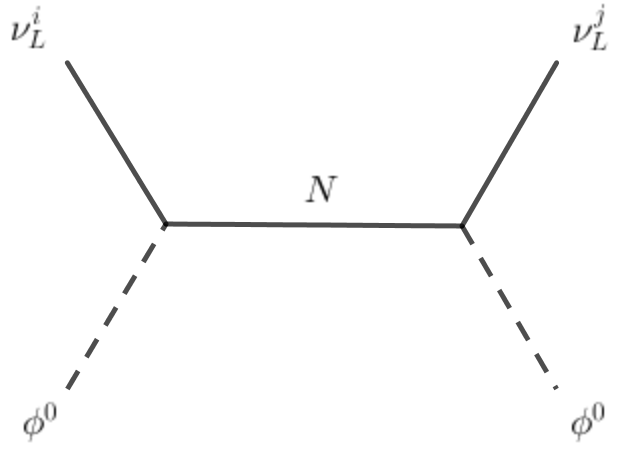
\includegraphics[width=0.4\linewidth]{dimension5operator}
  \caption{The tree level diagram which generates a Majorana mass term for the neutrinos after EWSB. This arises due to the introduction of a new heavy fermion $N$, which interacts with the neutrinos and the neutral Higgs scalar.}
  \label{fig:dimension5diag}
  \end{framed}
\end{figure}
\section{Linking Dark Matter and Majorana Neutrinos}
\subsection{Introduction to Dark Matter}
The fact that approximattely $23$\% of the universe at the current time is formed of non-baryonic matter generates a number of questions about the nature of this hidden sector;
\begin{enumerate}
  \item Is there a particle content to the sector, or is Dark Matter composite as in e.g. theories of Primordial Black Holes? \cite{Carr}
  \item Do we need physics beyond the Standard Model?
  \item If it does have a new particle content, how does this sector interact with the Standard Model?
  \item What evidence can be used to distinguish between and constriain different models?
\end{enumerate}
We are primarily interested in the last two questions posed, and will be considering extensions to the Standard Model. In particular we are concerned with phenomenological scenarios where the following two conditions hold;
\begin{itemize}
  \item The model contains a suitable dark matter candidate, in the sense that the particle is stable and whose interactions are not ruled out by the various astrophysical, thermal, collider, and cosmological bounds.
  \item The model \textit{also} contains a mechanism that generates the small Majorana neutrino mass. Whilst this is not necessary for the dark matter candidate to therefore be coupled directly to the Standard Model neutrinos, we will consider scenarios in which this is the case.
\end{itemize}
Of course, the last point is by no means a necessary requirement in a theory of dark matter, however the focus of this review is understanding to what extent we can build models that consistently, and naturally solve both issues.

Furthermore, we will spend a decent proportion of time later discussing the phenomenological consequences of both the low energy, and UV complete theories. Especially in the context of the effective low energy theory we present in Section \ref{sec:low energy theory}, any conclusions are greatly strengthened if they probe a parameter space not categorically ruled out by other bounds.
\subsection{Understanding the Role of $\mathbb{Z}_2$}\label{sec:understanding Z2}
One of the key properties mentioned above is that particle Dark Matter should be stable. In the majority of the rest of the review, we will claim that our Dark Matter candidate is stable ``as a result of a $\mathbb{Z}_2$ symmetry''. The aim of this section is to illustrate how this manifests itself within a UV extension to the Standard Model \cite{Ma2006a, Kubo2006, Ma2006, Ma2001}.

The big picture is as follows; we will introduce a new scalar into the Standard Model which will be odd under a new global $\mathbb{Z}_2$ symmetry. Through interactions with Standard Model neutrinos and new heavy fermions, it will generate a very similar dimension $5$ operator in a completely analogous way to the neutral Higgs field, $\phi^0$. Unlike the Higgs however, we shall see that the effect of the $\mathbb{Z}_2$ symmetry on the Higgs potential for the model ensures that the new scalar cannot develop a VEV. It also means that the lightest degree of freedom is rendered stable in a way to be explained further below. These two facts have the combined effect that (i) The neutrino mass is still generated in this process, but at one loop instead of at tree level, (ii) The lightest degree of freedom in the scalar sector is stable and can therefore act as our Dark Matter candidate.
\subsection{The Toy Model: $\SU{2}_L \times \Uni{1}_Y \times \mathbb{Z}_2$}
In what follows, one should bear in mind the case illustrated in \ref{sec:Tree Level Realisations of Majorana Masses} to compare which features are retained, and which features are constrained by the new $\mathbb{Z}_2$ symmetry. In particular, we will find that (i) an analogous dimension $5$ operator to $\phi^0 \phi^0 \nu^i_L \nu^j_L$ is generated, but, (ii) unlike the neutral component of the Higgs doublet, the new scalar will not acquire a VEV due to the $\mathbb{Z}_2$ symmetry. These two considerations along with an additional assumption regarding the lepton number of the new particle content will result in the neutrino masses only being generated at one loop.
\subsubsection{Particle Content}\label{sec:particle content}
Describing the particle content of the theory is equivalent to noting the different representations of the fields with respect to the group $\mathscr{H} = \SU{2}_L \times \Uni{1}_Y \times \mathbb{Z}_2$.\footnote{We are supressing the $\SU{3}_C$ part of the gauge group simply because in the sectors under consideration, all fields are in the trivial representation of $\SU{3}_C$.} In what follows, we shall use the following notation; consider some arbitrary field $\chi$, then we say that $\chi \sim (R_{\SU{2}}, R_{\Uni{1}}, R_{\mathbb{Z}_2})$ if;
\begin{itemize}
  \item $\chi$ is in the $R_{\SU{2}}$ representation of $\SU{2}$. For example, if $\chi$ were an $\SU{2}$ doublet, then we would take $R_{\SU{2}} = 2$ etc.
  \item $\chi$ has hypercharge $R_{\Uni{1}}$ with respect to $\Uni{1}_Y$, i.e. $\chi \rightarrow e^{iR_{\Uni{1}}\alpha}\chi$ under a $\Uni{1}_Y$ gauge transformation.
  \item $\chi$ has parity $R_{\mathbb{Z}_2}$ under $\mathbb{Z}_2$. For example, if $\chi$ were odd under $\mathbb{Z}_2$, then $R_{\mathbb{Z}_2} = -1$.
\end{itemize}
As an aside that we will use implicitly, a term in the Lagrangian is gauge invariant under transformations by elements of $\mathscr{H}$ if it lies in the trivial representation $(1, 1, +1)$. To check whether this is the case, by our definition, it is simply a matter of adding the respective $R$ values together for each field in the coupling. The particle content in the lepton and and scalar sectors is then as follows;
\begin{itemize}
  \item The three electroweak doublets, $\psi_i = (\nu^i_L, \ell^i_L)^{\textrm{T}} \sim (2, -\tfrac{1}{2}, +1)$, and the associated right-handed lepton fields, $\ell^i_R \sim (1, 1, +1)$;
  \item The Higgs electroweak doublet, $\Phi = (\phi^+, \phi^0)^{\textrm{T}} \sim (2, \tfrac{1}{2}, +1)$;
  \item The first new particle is a right-handed lepton, $N^i_R \sim (1, 0, -1)$, \textit{with lepton number} $l = 0$ \cite{Ma2001};
  \item A scalar electroweak doublet, $\eta = (\eta^+, \eta^0)^{\textrm{T}} \sim (2, \tfrac{1}{2}, -)$ with lepton number $l = -1$.
\end{itemize}
Note that the new particles are odd under the $\mathbb{Z}_2$ symmetry, whilst the Standard Model particles are even. Now, at this point, it is important to note why no term $\phi^0 \phi^0 \nu^i_l \nu^j_L$ can be generated in this model. As we saw in \ref{sec:Tree Level Realisations of Majorana Masses}, to generate such a term at tree level, we need a coupling of the form $\bar{N}^i_R(\nu^j_L \phi^0 - \ell_L \phi^+)$.\footnote{We will see where such a term comes from shortly} However, lepton number conservation forbids such a term, since $l(\bar{N}\nu\phi) = 0 + 1 + 0 = 1 \neq 0$. The absence of this term means that at tree level, we do not generate Majorana neutrino masses after EWSB.

On the other hand, the fact that $l(\eta) = -1$ means that an identical term with $\phi$ interchanged $\eta$ is not forbidden and will therefore generate an effective dimension $5$ operator $\Lambda^{-1}\eta^0 \eta^0 \nu^i_L \nu^j_L$ via a diagram like Figure \ref{fig:dimension5diag}. If $\eta^0$ were to acquire a VEV $\langle \eta^0 \rangle \neq 0$, this would generate neutrino mass at tree level. In the next few sections, we will see why this is not the case in this model.
\subsubsection{The Higgs Potential}
To begin we shall consider the most general $\SU{2} \times \Uni{1}$ invariant scalar Lagrangian. This will therefore necessarily include terms that break the $\mathbb{Z}_2$ symmetry explicitly. We will then derive the expected VEVs that arise from this general framework to understand why $\mathbb{Z}_2$ symmetry sets the $\eta^0$ VEV to zero. This will be equivalent to setting the couplings of the $\mathbb{Z}_2$-breaking terms to zero. The most general Higgs potential is of the form;
\begin{dmath}\label{eq:scalar lagrangian}
  V_s = m_1^2 \Phi\dagg \Phi + m_2^2 \eta\dagg \eta + \frac{1}{2}\lambda_1(\Phi\dagg\Phi)^2 + \frac{1}{2}\lambda_2(\eta\dagg\eta)^2 + \lambda_3 (\Phi\dagg\Phi)(\eta\dagg\eta) + \lambda_4 (\Phi\dagg\eta)(\eta\dagg\Phi) + \mu_{12}^2(\Phi\dagg\eta + \eta\dagg \Phi)
\end{dmath}
Note that only the last term expliclty breaks the $\mathbb{Z}_2$ symmetry, so moving to the $\mathbb{Z}_2$-symmetric case is equivalent to setting $\mu_{12}^2 = 0$ in the calculations that follow. To find show that the VEV of $\eta^0$ does indeed vanish for $\mu^2_{12} = 0$, we consider the constraint equations $\del_{\Phi}V_s = \del_{\eta}V_s = 0$. Letting $v$ and $u$ be the VEV of $\phi^0$ and $\eta^0$ respectively, we find \cite{Ma2001};
\begin{align}
  m_1^2 v + \lambda_1 v^3 + (\lambda_3 + \lambda_4)vu^2 + \mu^2_{12}u &= 0 \\
  m_2^2 u + \lambda_2 u^3 + (\lambda_3 + \lambda_4)uv^2 + \mu_{12}^2v &= 0
\end{align}
In the case that the Higgs field acquires a VEV, $m_1^2 < 0$, which of course certainly occurs, and we have $m_2^2 > 0$ with $\mu_{12}^2 \ll m_2^2$, we find that;
\begin{equation}
  v^2 \simeq -\frac{m_1^2}{\lambda_1}, \quad u \simeq -\frac{\mu_{12}^2 v}{m_2^2 + (\lambda_3 + \lambda_4)v^2}
\end{equation}
From this we immediately see that indeed if $\mu_{12}^2 = 0$, the VEV of $\eta^0$, $\langle \eta^0 \rangle = 0$. This has a couple of immediate consequences which will be discussed more in the next section;
\begin{enumerate}
  \item Although the coupling $\bar{N}^i_R \nu^j_L \eta^0$ arises in a gauge invariant manner, the fact that the VEV of $\eta^0$ vanishes implies that there is no Dirac mass linking $\nu^i_L$ and $N^i_R$.
  \item It also leads to the effect discussed above where the neutrinos do not acquire a mass at tree level, only at one loop.
\end{enumerate}
\subsubsection{Yukawa Sector}
Along with a Majorana mass term for the right-handed $N^i_R$ of the form;
\begin{equation}
  \frac{1}{2}M_{ij}N^i_R N^j_R + \text{h.c.}
\end{equation}
We also have a Yukawa sector of the Lagrangian that takes the form;
\begin{equation}
  \mL_{Y} = f_{ij}\Phi\dagg\psi^i \ell^j_R + h_{ij}\bar{\Psi}^i(i\sigma_2)\eta N^j + \text{h.c.}
\end{equation}
Where $\sigma_2$ is one of the Pauli matrices.\footnote{$$\sigma_2 = \twobytwo{0}{1}{-1}{0}$$} There are a couple of things to note about this Lagrangian;
\begin{itemize}
  \item Each of the terms is indeed gauge invariant under $\mathscr{H}$. For example the first term has a combined representation $(-2 + 2 + 1, -\tfrac{1}{2} + 1 - \tfrac{1}{2}, +1 \cdot +1 \cdot +1) = (1, 1, +1)$, and similarly for the second term.
  \item By expanding the definitions of $\Phi$ and $\psi^i$, as well as using the definitions of $\sigma_2$, we see exactly where the term of the form $h_{ij}(\nu^i_L \eta^0 - \ell^j_L \eta^+)N^j_R$ comes from. This term will then generate the effective vertex $\Lambda^{-1}\eta^0 \eta^0 \nu^i_L \nu^j_L$ discussed \ref{sec:Tree Level Realisations of Majorana Masses}.
\end{itemize}
\subsubsection{Generating Neutrino Mass}
To understand where the neutrino mass comes from in this model, we first make it clear that the Majorana mass does indeed still come from the effective operator $\phi^0 \phi^0 \nu^i_L \nu^j_L$. This ensures that after EWSB, the neutrino does acquire a mass. The point is however that this only happens at one loop. To see this, note;
\begin{itemize}
  \item There are $4$ point interactions in $V_s$ of the form $\lambda_3\Phi\dagg \Phi \eta\dagg\eta + \lambda_4 (\Phi\dagg \eta)(\eta\dagg \Phi)$ which are not prohibited by the $\mathbb{Z}_2$ symmetry.
  \item We have an interaction vertex in the Yukawa sector of the form $\bar{N}^i_R \eta^0 \nu^j_L $, which again is not prohibited by gauge invariance of violation of lepton number.
\end{itemize}
The combination of these two observations lead to a diagram of the form shown in Figure \ref{fig:oneloopmassdiag}. One can then use the associated Feynman rules to compute the value of the diagram and sum over the different neutrino species to obtain a mass matrix for the neutrinos below the electroweak scale. We will postpone this calculation until we consider a completely anaologous one in the next section.
\begin{figure}
  \begin{framed}
  \centering
  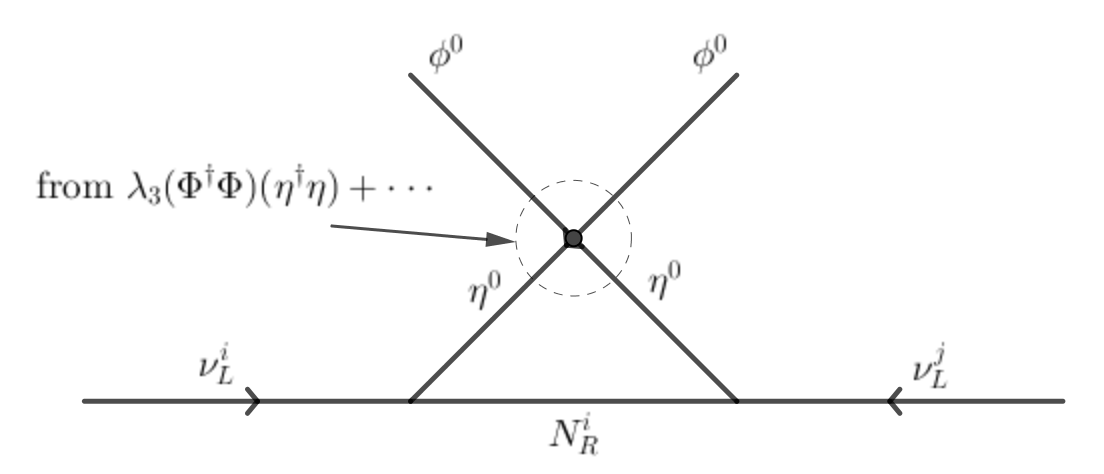
\includegraphics[width=0.6\linewidth]{oneloopmass}
  \caption{One loop diagram which radiatively generates the effective interaction $\phi^0\phi^0 \nu^i_L \nu^j_L$. This will lead to Majorana neutrino mass after EWSB, when $\langle \phi^0 \rangle = v$.}
  \label{fig:oneloopmassdiag}
  \end{framed}
\end{figure}
\subsubsection{Scalar Degrees of Freedom}
The only thing left is to investigate the Dark Matter candidate in the model \cite{Ma2006a}. To do so we should study the low energy scalar degrees of freedom. The correct regime to work in for the low energy spectrum is after EWSB. By gauge invariance, we can consider the Higgs doublet to take the form $\Phi = (0, v + \mathfrak{R}\phi^0)^{\text{T}}$ and expand the scalar Lagrangian in \eqref{eq:scalar lagrangian} using this ansatz. Firstly note that we have removed $\mathfrak{I}\phi^0$ using the residual gauge freedom. The remaining physical scalar degrees of freedom are then;
\begin{equation}
  \mathfrak{R}\phi^0, \quad \eta^{\pm}, \quad \mathfrak{R}\eta^0, \quad \mathfrak{I}\eta^0
\end{equation}
By expanding the Lagrangian and collecting together the quadratic terms, we find;
\begin{dmath}
  V_s = m_1^2 (\mathfrak{R}\phi^0)^2 + \frac{1}{2}m_2^2 \left((\mathfrak{R}\eta^0)^2 + (\mathfrak{I}\eta^0)^2 + (\eta^+)^2 + (\eta^-)^2\right) + \lambda_1 (\mathfrak{R}\phi^0)^2 + \lambda_2v^2 \left((\mathfrak{R}\eta^0)^2 + (\mathfrak{I}\eta^0)^2 + (\eta^+)^2 + (\eta^-)^2\right) + \lambda_3v^2 \left((\mathfrak{R}\eta^0)^2 + (\mathfrak{I}\eta^0)^2\right) + \lambda_4v^2 \left((\mathfrak{R}\eta^0)^2 - (\mathfrak{I}\eta^0)^2\right) + \text{non mass terms}
\end{dmath}
From this we can read off the masses of the physical degrees of freedom;
\begin{itemize}
  \item $m^2(\sqrt{2}\mathfrak{R}\phi^0) = 2\lambda_1 v^2$, using the relationship $v^2 = -m_1^2/\lambda_1$
  \item $m^2(\eta^{\pm}) = m_2^2 + \lambda_3 v^2$
  \item $m^2(\sqrt{2}\mathfrak{R}\eta^0) = m_2^2 + (\lambda_3 + \lambda_4 + \lambda_5)v^2$
  \item $m^2(\sqrt{2}\mathfrak{I}\eta^0) = m_2^2 + (\lambda_3 + \lambda_4 - \lambda_5)v^2$
\end{itemize}
We are now in a position to make the conclusion that, depending on the sign of $\lambda_5$ and suitable choices for the other parameters, either $\mathfrak{R}\eta^0$ or $\mathfrak{I}\eta^0$ is the lightest stable particle. Again, we emphasise that this is stabilised by the $\mathbb{Z}_2$ symmetry. To see this imagine a diagram with one external $\mathfrak{R}/\mathfrak{I}\eta^0$ leg. The Ward identity for the $\mathbb{Z}_2$ symmetry prohibits any decay into a final state that has none of the Dark Matter candidate particle. Hence it is stable to decay in this sense.

\section{The Low Energy Effective Field Theory}\label{sec:low energy theory}
The discussion of UV complete theories presents a concrete scenario to implement the ideas of radiatively generating neutrino mass, as well as providing a dark matter candidate. On the other hand, at a given low energy scale, our experiments will not be able to probe the UV structure of the theory, only the effective degrees of freedom remaining at the scale in question (e.g. the energy scale at the LHC, or in cosmological scenarios). This is ultimately a statement about renormalisation flow in that we can construct a number of UV theories whose low energy degrees of freedom nonetheless appear to be the same.

In this section, we will present a low energy effective theory that contains a scalar Dark Matter candidate coupled to neutrinos \cite{Farzan2014, Farzan2011, Farzan2010, Boehm2006, Farzan2009} that generates a one-loop neutrino mass. This will include a discussion of both real and complex scalars, since the two have qualitatively different constraints. We shall explain why it must be an effective theory, as well as how the neutrino mass is generated. More importantly, we will focus on the phenomenological consequences of the model and be as clear as possible as to exactly what constraints these place on the couplings and masses within the theory. These include astrophsyical, particle physics, and cosmological bounds \cite{Farzan2014, Farzan2011, Farzan2010, Boehm2006, Farzan2009}. This will provide the basis for further numerical investigation.

This is not to say that providing a clear embedding of the low energy theory is not useful at all. Indeed in Section \ref{sec:UV completions}, we will provide a review of one way to embed the dark matter candidate in a UV theory to illustrate where the relevant degrees of freedom may come from \cite{Farzan2009, Farzan2010a}. Furthermore, we will also discuss the possible phenomenological implications of these \textit{UV theories}, although necessarily the bounds they imply must be weaker than in the effective field theory case.
\subsection{The Lagrangian and Particle Content}
The overarching motivation for this work is that whatever model we consider should link neutrino mass generation and scalar dark matter particle content. In this regard, our focus is on a low energy particle spectrum that consists of the Standard Model along with;
\begin{itemize}
  \item A scalar field, $\delta$, which may be real or complex;
  \item Two or more massive right-handed fermions $N^i_R$, note that this is not the same fermion as in Section \ref{sec:particle content}, but it is consistent across the literature.
\end{itemize}
In addition to this, we assume that there is a residual $\mathbb{Z}_2$ symmetry under which the new particles are odd, and the Standard Model is even. This has a number of effects, in a fashion completely analagous to the discussion in Section \ref{sec:understanding Z2};
\begin{enumerate}
  \item It ensures that the lightest particle in the spectrum is stable, providing a Dark Matter candidate
  \item It prohibits a term of the form $\phi^0 \bar{N}_R^i \nu^\alpha_L$, so that after EWSB, there is no Dirac mass term linking $N^i_R$ and $\nu^\alpha_L$. This means that the neutrino mass is not generated at tree level.
  \item The new scalar, $\delta$, cannot acquire a VEV, due to the structure of the Higgs sector
\end{enumerate}
The key feature we are interested in however is the interaction part of the Lagrangian which couples this new dark sector to the neutrino sector in the Standard Model. In our effective theory, we take the couplings to be of the form;
\begin{framed}
\begin{equation}\label{eq:effective lagrangian}
  g_{i\alpha}\delta \bar{N}^i_R \nu^\alpha_L + \text{h.c.}
\end{equation}
\end{framed}
\noindent Where there is an implicit sum over the right-handed fermion species, $i$, and the Standard Model neutrino species, $\alpha$. Later we will be interested in constraining the values of the coupling constants.
\subsubsection{Why must it be an effective theory?}\label{sec:why effective}
To understand why the Lagrangian in \eqref{eq:effective lagrangian} must be effective, i.e. only valid up to some high energy scale $\Lambda$, we make an assumption regarding the representations of the new fields. We assume that there are no electroweak interactions between $\delta$, $N^i_R$ and the electroweak gauge bosons. In other words, they lie in the trivial representation of $\SU{2}_L \times \Uni{1}_Y$. This is important because the Standard Model neutrinos are charged under the electroweak symmetry. Therefore the coupling in \eqref{eq:effective lagrangian} cannot be gauge invariant. It must therefore be an effective theory that is part of some $\SU{2}_L \times \Uni{1}_Y$ invariant UV theory. The implication of this is that when we calculate for example loop diagrams, we should bear in mind that the theory does not hold up to arbitrarily high energies. Instead there is some cutoff, $\Lambda$, below which our Lagrangian is a valid description.
\subsection{Generation of Neutrino Masses}
In this section we will explicitly calculate the contribution to the neutrino mass matrix that arises due to interaction term in \eqref{eq:effective lagrangian}. The Majorana mass term for the neutrino is of the form;
\begin{equation}\label{eq:neutrino mass}
  \frac{1}{2}(m_\nu)_{\alpha\beta}\left(\bar{\nu}^\alpha_L \nu^\beta_L + \text{h.c.}\right)
\end{equation}
We are interested in calculating the mass matrix $(m_\nu)_{\alpha\beta}$. To do so, we will need to distinguish between the two cases where either (i) $\delta$ is a real scalar field, or, (ii) $\delta$ is a complex scalar field.
\subsubsection{Case 1: Real Scalar Field}
In this case, there is only one diagram that contributes to the neutrino mass, as shown in Figure \ref{fig:onelooprealdiag}. We note a couple of points regarding the the diagram;
\begin{itemize}
  \item Any of the species of right-handed fermion $N^i_R$ can run around the loop, so we should sum over these possibilities
  \item As indicated, the diagram should be evaluated at zero external momenta. This is in order to extract only the mass contribution. For non-zero external momenta, there would also generically be higher order\footnote{Higher order in the sense of derivates, the terms will still be quadratic in the neutrino fields.} derivative terms generated by the loop integral.
\end{itemize}
With this in mind, the contribution to the neutrino mass is given by;
\begin{dmath}\label{eq:oneloopmasseq}
  \frac{1}{2}(m_\nu)_{\alpha \beta} = \sum_{i}{g_{i\alpha}g_{i\beta}\int^{\Lambda}\left.{\frac{\ud^4 p}{(2\pi)^4}\frac{\slashed{p} - \slashed{k} + m_{N^i}}{\left((p - k)^2 - m_{N^i}^2\right)(p^2 - m_\delta^2)}}\right|_{k = 0}}
\end{dmath}
\begin{figure}
  \begin{framed}
  \centering
  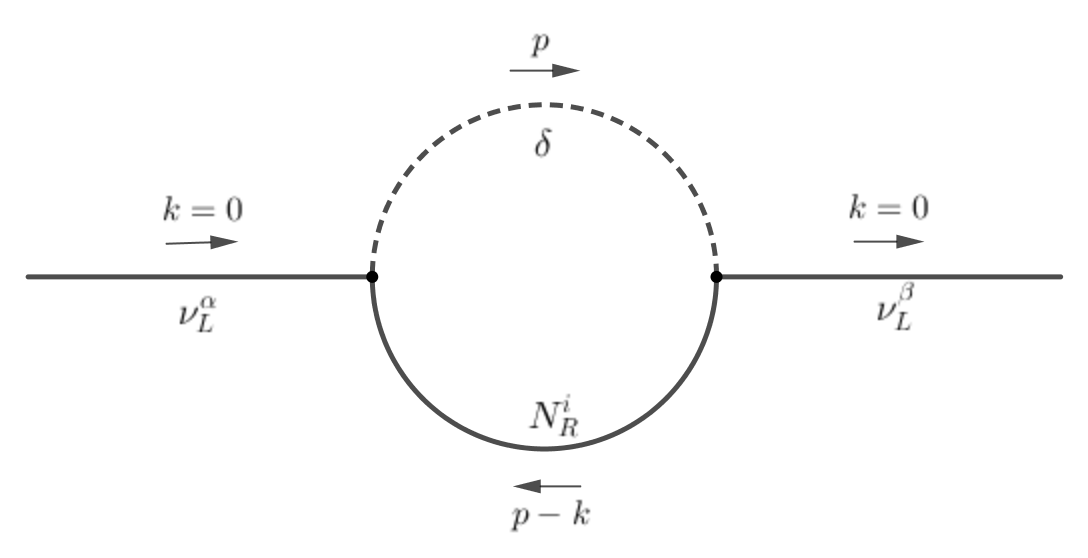
\includegraphics[width=0.7\linewidth]{oneloopreal}
  \caption{The one loop diagram contributing to the neutrino mass in the case that $\delta$ is a real scalar. The external neutrinos are evaluated at zero incoming momenta so as to extract only the mass contribution as opposed to the quadratic derivative interactions.}
  \label{fig:onelooprealdiag}
  \end{framed}
\end{figure}
Note that the factor of $\tfrac{1}{2}$ in this formula comes from the same factor in \eqref{eq:neutrino mass}. To evaluate this first note that the term involving $\slashed{p}$ is odd in $p$ so when it is integrated over the full space, it vanishes. This leaves only terms of the schematic form;
\begin{equation}
  g_{i\alpha}g_{i\beta}\int^{\Lambda}{\frac{\ud^4 p}{(2\pi)^4}\frac{m_{N^i}}{\left(p^2 - m_{N^i}^2\right)(p^2 - m_\delta^2)}}
\end{equation}
We can compute the integral as follows, noting in particular the explicit dependence on the cutoff of the effective theory, $\Lambda$;
\begin{align*}
  \int^{\Lambda}{\frac{\ud^4 p}{(2\pi)^4}\frac{1}{\left(p^2 - m_{N^i}^2\right)(p^2 - m_\delta^2)}} &= \frac{\text{Vol}(S^3)}{32\pi^4}\int_{0}^{\Lambda}{p^3 \upd{p} \frac{1}{\left(p^2 - m_{N^i}^2\right)(p^2 - m_\delta^2)}} \\
  &= \frac{1}{16\pi^2}\int_{0}^{\Lambda}{p^3 \upd{p} \frac{1}{\left(p^2 - m_{N^i}^2\right)(p^2 - m_\delta^2)}}
\end{align*}
Now;
\begin{dmath}
  \frac{1}{16\pi^2}\int_{0}^{\Lambda}{p^3 \upd{p} \frac{1}{\left(p^2 - m_{N^i}^2\right)(p^2 - m_\delta^2)}} = \frac{1}{32\pi^2(m_{N^i}^2 - m_\delta^2)}\left(m_{N^i}^2 \log(\Lambda^2 - m_{N^i}^2) - m_{N^i}^2 \log m_{N^i}^2 - m_\delta^2 \log(\Lambda^2 - m_\delta^2) + m_\delta^2 \log m_\delta^2\right)
\end{dmath}
We now assume that our effective scale, which is likely above the electroweak scale, satisfies $Lambda \gg m_{N^i}, m_\delta$. In this case, we can simplify this to;
\begin{dmath}
\frac{1}{32\pi^2(m_{N^i}^2 - m_\delta^2)}\left(m_{N^i}^2 \log\Lambda^2 - m_{N^i}^2 \log m_{N^i}^2 - m_\delta^2 \log\Lambda^2 + m_\delta^2 \log m_\delta^2\right) = \frac{1}{32\pi^2(m_{N^i}^2 - m_\delta^2)} \left((m_{N^i}^2 - m_\delta^2)\log \frac{\Lambda^2}{m_{N^i}^2} - m_\phi^2 \log\frac{m_{N^i}^2}{m_\phi^2}\right)
\end{dmath}
We can now put this together with the expression in \eqref{eq:oneloopmasseq} to find the result quoted in \cite{Farzan2010, Boehm2006, Farzan2011};
\begin{equation}\label{eq:oneloopmass result}
  (m_\nu)_{\alpha\beta} = \sum_{i}{\frac{g_{i\alpha}g_{i\beta}}{16\pi^2}m_{N^i}\left(\log\frac{\Lambda^2}{m_{N^i}^2} - \frac{m_\delta^2}{m_{N^i}^2 - m_\delta^2}\log\frac{m_{N^i}^2}{m_\delta^2}\right)}
\end{equation}
\subsubsection{Case 2: Complex Scalar Field}
To investigate the complex scalar field, we should first think about the scalar degrees of freedom. Since the field is in the trivial representation of the electroweak gauge group, the most general hermitian mass term for $\delta$ can be written as \cite{Farzan2010};
\begin{equation}
  V_m = M^2 \delta\dagg \delta - \frac{1}{2}(m^2 \delta\delta + \text{h.c.})
\end{equation}
Consider expanding the scalar field as $\delta = \tfrac{1}{\sqrt{2}}(\delta_1 + i\delta_2)$ where $\delta_{1,2}$ are both real fields. Expanding the terms above in terms of these real degrees of freedom;
\begin{dmath}
  V_m = \frac{1}{2}M^2(\delta_1 + i\delta_2)(\delta_1 - i\delta_2) - \frac{1}{4}m^2\left((\delta_1 + i\delta_2)(\delta_1 + i\delta_2) + (\delta_1 - i\delta_2)(\delta_1 - i\delta_2)\right)
\end{dmath}
Collecting the terms together for each field we find;
\begin{equation}
  V_m = \frac{1}{2}(M^2 - m^2)\delta_1^2 + \frac{1}{2}(M^2 + m^2)\delta_2^2
\end{equation}
We can then immediately see that the mass eigenstates are simply $\delta_1$ and $\delta_2$ themselves, with masses $m^2_{\delta_1} = M^2 - m^2$, $m^2_{\delta_2} = M^2 + m^2$. The lighter of these will be our Dark Matter candidate. Before we do eventually calculate the neutrino mass in this case, we note that interaction term \eqref{eq:effective lagrangian} is diagonal in this mass basis;
\begin{equation}
  \mL_{\text{int}} = g_{i\alpha}\bar{N}^i_R \nu^\alpha_L (\delta_1 + i \delta_2)
\end{equation}
The contributions to the neutrino mass are then two diagrams of the form in Figure \ref{fig:onelooprealdiag}. One will have $\delta_1$ running round the loop, whilst the other will have $\delta_2$. We note that the only difference between them is that the second diagram will have two couplings with an extra factor of $i$, $(ig_{i\alpha})(ig_{i\beta}) = -g_{i\alpha}g_{i\beta}$. As such the second will come with a negative sign. The total contribution is then a sum of two contributions of the form \eqref{eq:eq:oneloopmass result};
\begin{dmath}
  (m_\nu)_{\alpha\beta} = \sum_{i}{\frac{g_{i\alpha}g_{i\beta}}{16\pi^2}m_{N^i}\left(\log\frac{\Lambda^2}{m_{N^i}^2} - \frac{m_{\delta_1}^2}{m_{N^i}^2 - m_{\delta_1}^2}\log\frac{m_{N^i}^2}{m_{\delta_1}^2}\right)} - \sum_{i}{\frac{g_{i\alpha}g_{i\beta}}{16\pi^2}m_{N^i}\left(\log\frac{\Lambda^2}{m_{N^i}^2} - \frac{m_{\delta_2}^2}{m_{N^i}^2 - m_{\delta_2}^2}\log\frac{m_{N^i}^2}{m_{\delta_2}^2}\right)}
\end{dmath}
Importantly, we see that the dependence on the cutoff drops out in the complex case and we find;
\begin{equation}
  (m_\nu)_{\alpha\beta} = \sum_{i}{\frac{g_{i\alpha}g_{i\beta}}{16\pi^2}m_{N^i}\left(\frac{m_{\delta_2}^2}{m_{N^i}^2 - m_{\delta_2}^2}\log\frac{m_{N^i}^2}{m_{\delta_2}^2} - \frac{m_{\delta_1}^2}{m_{N^i}^2 - m_{\delta_1}^2}\log\frac{m_{N^i}^2}{m_{\delta_1}^2}\right)}
\end{equation}
\subsection{Astrophysical, Cosmological, and Particle Physics Constraints}
So far we have illustrated (i) how neutrino mass is generated within the effective framework, and, (ii) discussed which are the relevant degrees of freedom when it comes to suitable dark matter candidates. We now discuss the vital question as to what constraints have already been placed on the model across a range of scenarios. We will investigate the constraints that arise from the two key scenarios \cite{Boehm2006, Franarin2018, Farzan2009, Farzan2011, Farzan2014, Farzan2010};
\begin{enumerate}
  \item The cosmological bound on the Dark Matter annihilation cross section;
  \item The bounds that arise due to light meson and tau decay.
\end{enumerate}
We will also discuss some of the other astrophysical bounds in slightly more general terms.
\subsubsection{Dark Matter Annihilation Cross Section}
Within this effective model, there are three annihilation channels in the case that $N^i_R$ is a Majorana fermion, given by $\delta \delta \rightarrow \set{\nu\nu, \nu\bar{\nu}, \bar{\nu}\bar{\nu}}$. According to \cite{Boehm2006}, the cross section for the process $\delta\delta \rightarrow \nu\bar{\nu}$ is suppresed relative to the other two, so we consider just those. Suppressing somewhat the distinction between the different flavours of neutrinos, as well as the different types of new fermion, the thermally averaged cross section is given by \cite{Boehm2006};
\begin{equation}
  \langle \sigma v \rangle \simeq 2\langle\sigma(\delta\delta \rightarrow \nu \nu) \rangle \simeq \frac{g^4}{4\pi}\frac{m_N^2}{(m_\delta^2 + m_N^2)^2}
\end{equation}
Note that this implies that;
\begin{dmath}\label{eq:mN}
  m_N^2 \simeq \frac{2\pi}{g^4}(m_\delta^2 + m_N^2)^2 \langle \sigma v \rangle \Rightarrow m_N \nobreak \simeq \frac{\sqrt{2\pi}}{g^2}(m_\delta^2 + m_N^2)\sqrt{\langle\sigma v\rangle}
\end{dmath}
\subsubsection*{Real Scalar Dark Matter}
In the real case, we make a simplification that the first term in \eqref{eq:oneloopmass result} dominates, then we can use \eqref{eq:mN} to approximate;
\begin{equation}
  m_{\nu} \simeq \frac{g^2 m_N}{16\pi^2}\log \frac{\Lambda^2}{m_N^2} \simeq \frac{g^2}{16\pi^2}\sqrt{2\pi\langle\sigma v\rangle}\frac{1}{g^2}(m_\delta^2 + m_N^2)\log\frac{\Lambda^2}{m_N^2}
\end{equation}
The rationale behind this is that after simplifying the expression above, we have removed the dependence on $g$. We see that;
\begin{equation}
  m_\nu \simeq \sqrt{\frac{\langle\sigma v\rangle}{128\pi^3}}m_N^2 \left(1 + \frac{m_\delta^2}{m_N^2}\right)\log\frac{\Lambda^2}{m_N^2}
\end{equation}
We can take a number of key insights from this relation;
\begin{itemize}
  \item The neutrino mass is very closely related to the Dark Matter abundance, since this is determined at freeze out in terms of the annihilation cross section;
  \item We have some bound on $m_\nu$ from neutrino experiments and Cosmology;
  \item $\langle\sigma v \rangle$ is set by the requirement that the relic density of Dark Matter agrees with the observed value;
  \item The free parameters in the model are $m_N$, $m_\delta/m_N$, and $\Lambda$. However note that (i) $m_\delta/m_N \in [0, 1]$ in order that $\delta$ remains the lightest particle and hence the Dark Matter candidate, (ii) the dependence on $\Lambda$ is logarithmic. We deduce that $m_N$ is therfore the most important parameter.
\end{itemize}
Finally then, we take \cite{Boehm2006} $\Lambda \sim 200 \, \text{GeV}$, $0.01 \, \text{eV} < m_\nu < 1\, \text{eV}$ and the fact that sub-GeV Dark Matter requires $\langle \sigma v \rangle \simeq 10^{-26}\, \text{cm}^3\text{s}^{-1}$. This allows us to read off bounds on the mass of;
\begin{framed}
\begin{equation}
  \mO(1 \, \text{MeV}) \lesssim m_\phi < m_N \lesssim 10 \, \text{MeV}
\end{equation}
\end{framed}
\noindent Notice that this bound can be reduced by increasing the precision of the neutrino mass. Rearanging for the coupling, we find;
\begin{equation}
  g \simeq 10^{-3}\sqrt{\frac{m_N}{10 \, \text{MeV}}}\left(\frac{\langle\sigma v\rangle}{10^{-26} \, \text{cm}^3 \text{s}^{-1}}\right)^{\frac{1}{4}}\left(1 + \frac{m_\delta^2}{m_N^2}\right)^{\frac{1}{2}}
\end{equation}
With the range of neutrino masses chosen, we find the bound;
\begin{framed}
\begin{equation}
3 \times 10^{-4} \lesssim g \lesssim 10^{-3}
\end{equation}
\end{framed}
\subsubsection*{Complex Scalar Dark Matter}
In the complex case, we can apply a similar idea, except that the correction to the neutrino mass is now given by;
\begin{equation}
  (m_\nu)_{\alpha\beta} \simeq \frac{g^2}{16\pi^2}m_{N}\left(\frac{m_{\delta_2}^2}{m_{N}^2 - m_{\delta_2}^2}\log\frac{m_{N}^2}{m_{\delta_2}^2} - \frac{m_{\delta_1}^2}{m_{N}^2 - m_{\delta_1}^2}\log\frac{m_{N}^2}{m_{\delta_1}^2}\right)
\end{equation}
Making the same substitution for the $m_N$ prefactor in terms of the annihilation cross-section, we find;
\begin{equation}
  m_\nu \simeq \sqrt{\frac{\langle \sigma v \rangle}{128\pi^3}}\left(m_{\delta_2}^2 \log\frac{m_{N}^2}{m_{\delta_2}^2} - m_{\delta_1}^2\log\frac{m_{N}^2}{m_{\delta_1}^2}\right)
\end{equation}
Now we can make a similar deduction by varying the neutrino mass to find in this scenario;
\begin{framed}
  \begin{equation}
    (1\, \text{MeV})^2 \lesssim \Abs{m_{\delta_2}^2 - m_{\delta_1}^2} \lesssim (20 \, \text{MeV})^2
  \end{equation}
\end{framed}
\noindent We note that now $m_N$ is a free parameter, so is far less constrained than in the real case. In turn, this implies that $g$ is less constrained to be so weak, although we shall see that there are different bounds due to light meson decay. As a final comment on this scenario, we do note that although the masses of the scalars are not necessarily constrained, the mass difference is $\mO(\text{MeV})$, suggesting on naturalness grounds, that the masses themselves are probably of a similar order.
\subsubsection{Light Meson and Tau Decay}
Consider the decay $A \rightarrow B + \nu$ \cite{Farzan2011, Farzan2014, Farzan2010}, then generically if the coupling in \eqref{eq:effective lagrangian} is present, eventually $\nu \rightarrow N^i_R \delta$. This means we should see $A \rightarrow B + \text{missing energy}$. To see how this provides bounds on the couplings, we shall provide the specific example of kaon decay. We will then quote the generic bounds found in the literature due to this process in the context of other decay channels. Consider the ratio;
\begin{equation}
  \frac{\Gamma(K^+ \rightarrow e^+ + \text{missing energy})}{\Gamma(K^+ \rightarrow \mu^+ + \text{missing energy})} = \frac{\Gamma_{\text{SM}}(K^+ \rightarrow e^+ \nu_e) + \sum_{i}{\Gamma(K^+ \rightarrow e^+ N^i_R \delta)}}{\Gamma_{\text{SM}}(K^+ \rightarrow \mu^+ \nu_e) + \sum_{i}{\Gamma(K^+ \rightarrow \mu^+ N^i_R \delta)}}
\end{equation}
Note that we can rearrange this as the ratio;
\begin{equation}
  \frac{\frac{\Gamma_{\text{SM}}(K^+ \rightarrow e^+ \nu_e)}{\Gamma_{\text{SM}}(K^+ \rightarrow \mu^+ \nu_e)} + \sum_{i}{\frac{\Gamma(K^+ \rightarrow e^+ N^i_R \delta)}{\Gamma_{\text{SM}}(K^+ \rightarrow \mu^+ \nu_e)}}}{1 + \sum_{i}{\frac{\Gamma(K^+ \rightarrow \mu^+ N^i_R \delta)}{\Gamma_{\text{SM}}(K^+ \rightarrow \mu^+ \nu_e)}}}
\end{equation}
Now the restricted phase space for the decay $K^+ \rightarrow \mu^+ N^i_R \delta$ compared to $K^+ \rightarrow \mu^+ \nu_e$ ensures that;
\begin{equation}
  \frac{\Gamma(K^+ \rightarrow \mu^+ N^i_R \delta)}{\Gamma_{\text{SM}}(K^+ \rightarrow \mu^+ \nu_e)} \ll 1
\end{equation}
So we can approximate;
\begin{equation}
  \frac{\Gamma(K^+ \rightarrow e^+ + \text{missing energy})}{\Gamma(K^+ \rightarrow \mu^+ + \text{missing energy})} \simeq \frac{\Gamma_{\text{SM}}(K^+ \rightarrow e^+ \nu_e) + \sum_{i}{\Gamma(K^+ \rightarrow e^+ N^i_R \delta)}}{\Gamma_{\text{SM}}(K^+ \rightarrow \mu^+ \nu_e)}
\end{equation}
This is an important simplification in the sense that the new ratio depends on only one of the couplings, in this case $g_{ie}$. Experiments such as KLOE \cite{Ambrosino2009} can constrain this ratio. The most recent constraints give;
\begin{framed}
  \begin{equation}
    \sum_{i}{\Abs{g_{ie}}^2} < 10^{-5}
  \end{equation}
\end{framed}
\noindent We can use the same methodology for $K^+ \rightarrow \mu^+ + \text{missing energy}$ to constrain the $g_{i\mu}$ couplings. In this case, the results come from \cite{Artamonov2016} the LBL Bevatron;
\begin{framed}
  \begin{equation}
    \sum_{i}{\Abs{g_{i\mu}}^2} \lesssim 10^{-4}
  \end{equation}
\end{framed}
\noindent Finally, by considering decays such as $\tau \rightarrow \mu \nu N^i_R \delta$ \cite{Farzan2010}, we can put constraints on the tau coupling, although these are much weaker;
\begin{framed}
  \begin{equation}
    \sum_{i}{\Abs{g_{i\tau}}^2} < 10^{-1}
  \end{equation}
\end{framed}
\noindent There are a couple of important observations that need to be made with respect to these bounds;
\begin{itemize}
  \item Provided $\max(m_\delta^2, m_{N^i}^2) \ll m_{K, \pi} \simeq \mO(500\,\text{MeV})$, the bounds are similar in both the complex and the real case;
  \item With the bounds as above, we note that the couplings themselves can have magnitudes;
  \begin{equation}
    \Abs{g_{ie}} \lesssim 3 \times 10^{-3}, \quad \Abs{g_{i\mu}} \lesssim 10^{-2}, \quad \Abs{g_{i\tau}} \lesssim 3 \times 10^{-1}
  \end{equation}
  \item In the heavy case \cite{Farzan2014}, $m_K < m_\delta + m_{N^i} < m_D$, where $m_D$ is the mass of the $D$ meson, the bounds above do not apply. Instead the strongest bounds have $\Abs{g_{ie}} \lesssim 0.4$ and $g_{i\mu} \lesssim \mO(1)$.
\end{itemize}
\subsubsection{Additional Constraints}
The two methods of constraining the effective theory given above provide the most stringent bounds on the couplings and the masses. Furthermore, they also provide two very distinct scenarios for comparison. The first investigates the phenomenology in the setting of thermalizing early universe cosmology, whilst the second is a pure particle physics test. Within the literature \cite{Farzan2010, Boehm2006}, there are a couple of other suggestions for additional, or future methods of constraint. These include;
\begin{enumerate}
  \item \textit{Supernova Core Collapse:} It is suggested \cite{Franarin2018, Farzan2010} that we could search for a dip in the neutrino energy spectrum coming from neutrinos produced during supernova core collapse.
  \item \textit{Large Scale Structure:} This places constraints on the mass \cite{Boehm2004} due to the damping length of $m \lesssim \mO(\text{keV})$.
  \item \textit{Big Bang Nucleosynthesis:} This can restrict the masses of the particles \cite{Boehm2006} due to the fact that baryon-to-photon ratio and light element abundance measurements place an upper bound on the number of additional degrees of freedom below the $\text{MeV}$ scale.\footnote{To be more precise, combinations of CMB, baryon-to-photon ratio, and light element abundance data place an upper bound of an additional $1.5$ degrees of freedom at the $95$\% confidence level.}
  \item \textit{Detection at Neutrino Experiments:} This is more of future work, but there is a suggestion \cite{Farzan2010} that experiments such as IceCube may be able generate constraints.
\end{enumerate}
\section{UV Completions of the Effective Model} \label{sec:UV completions}
In the last section, we studied the effective field theory and the observational constraints on it. We will spend the remainder of the review providing a concrete realisation of two UV completions of the effective Lagrangian; one for the real case, and the other for the complex scalar field. The two models will be qualitatively different, with a different particle content. We will also consider breifly some of the possible phenomenology, although we emphasise that the key constraints lie within the effective theory that will ultimately be the focus of any future work.
\subsection{Real Scalar Dark Matter}
As we explained in Section \ref{sec:why effective}, the effective theory is not $\SU{2} \times \Uni{1}$ invariant. We must therefore embed this in an $\SU{2} \times \Uni{1}$ invariant UV completion. As we have done across the different settings, we also include a $\mathbb{Z}_2$ symmetry under which the new particles introduced below are odd, and Standard Model particles are even. The new particle content is as follows \cite{Farzan2009, Farzan2011};
\begin{itemize}
  \item An electroweak singlet $\chi$;
  \item Two Majorana fermions, $E^i$;
  \item An electroweak doublet $\Psi^{\text{T}} = (\psi^0, \psi^-)$ where $\psi^0 = \tfrac{1}{\sqrt{2}}(\psi_1 + i\psi_2)$
\end{itemize}
In the scalar sector, we also have the Higgs doublet $\Phi$, then the most general $\SU{2} \times \Uni{1}$ invariant, renormalisable Lagrangian is given by;
\begin{dmath}
  \mL_s = -m_\Psi^2 \Psi\dagg \Psi - \frac{m_s^2}{2}\chi^2 - (m_{\chi\Psi}\chi \Phi^{\text{T}}(i\sigma_2)\Psi + \text{h.c.}) - \lambda_1 (\Phi^{\text{T}}(i\sigma_2)\Psi)^2 - \mathscr{R}[\lambda_2(\Phi^{\text{T}}(i\sigma_2)\Psi)^2] - \lambda_3 \chi^2 \Phi\dagg \Phi - \lambda_4 \Psi\dagg \Psi \Phi\dagg \Phi - \frac{\lambda_1^{\prime}}{2}(\Psi\dagg\Psi)^2 - \frac{\lambda_2^{\prime}}{2}\chi^4 - \lambda_3^{\prime}\chi^2 \Psi\dagg\Psi - m_H^2 \Phi\dagg \Phi - \frac{\lambda}{2}(\Phi\dagg \Phi)^2
\end{dmath}
There are conditions for stability at large field values that arise from setting e.g. all fields except $\Phi$ to zero. These conditions are given by \cite{Farzan2009};
\begin{equation}
  \lambda_1^{\prime}, \lambda_2^{\prime} > 0, \quad \lambda_3^{\prime} > -\sqrt{\lambda_1^{\prime}\lambda_2^{\prime}}, \quad \lambda_3 > -\sqrt{\lambda\lambda_2^{\prime}}, \quad \lambda_1 - \Abs{\lambda_2} + \lambda_4 > -\sqrt{\lambda \lambda_1^{\prime}}
\end{equation}
WE also have a Yukawa sector which couples the Standard Model neutrinos to the new scalars and the new fermions. If we let $L^\alpha = (\nu^\alpha, \ell^\alpha)_L$ be the Standard Model lepton doublet, then the most general gauge invariant Yukawa Lagrangian is;
\begin{equation}
  \mL_Y = -h_{i\alpha}\bar{E}^i \Psi^\dagg L^\alpha - \frac{M_{ij}}{2}\bar{E}^i E^j
\end{equation}
where the second term encodes the Majorana mass of the new fermions.
\subsubsection{The Low Energy Spectrum}
To relate this to the effective field theory, we need to derive the low energy spectrum i.e. the masses of the relevant degrees of freedom. To do this, we recall that due to the $\mathbb{Z}_2$ symmetry, the new scalar cannot acquire a VEV, as such the relevant process to consider is EWSB where the Higgs doublet can be written as $\Phi = (0, \tfrac{v_H}{\sqrt{2}})$. The relevant mass terms in the scalar Lagrangian after spontaneous symmetry breaking are then;
\begin{dmath}
  \mL_m = -m_{\psi^-}^2 \Abs{\psi^-}^2 - \frac{m_{\psi_2}^2}{2}\psi_2^2 - \frac{m_\chi^2}{2}\chi^2 - \frac{m_{\psi_1}^2}{2}\psi_1^2 - m_{\chi\Psi}v_H \psi_1 \chi + \text{non mass terms}
\end{dmath}
To derive this, we simply extract the terms quadratic in the fields in the scalar Lagrangian, which will include contributions from quartic terms that contain two Higgs doublets for example. The parameters above can be related to the ones in the high energy Lagrangian via;\footnote{A techinicality that is considered in \cite{Farzan2009} is that we should tune the parameters to avoid also spontaneously breaking the $\mathbb{Z}_2$ symmetry.}
\begin{align}
  m_{\psi^-}^2 &= m_{\Psi}^2 + \lambda_4 \frac{v_H^2}{2} \\
  m_\chi^2 &= m_{\Psi}^2 + \lambda_3 \frac{v_H^2}{2} \\
  m_{\psi_1}^2 &= m_{\Psi}^2 + \lambda_1 \frac{v_H^2}{2} + \lambda_2 \frac{v_H^2}{2} \\
  m_{\psi_2}^2 &= m_{\Psi}^2 + \lambda_1 \frac{v_H^2}{2} - \lambda_2 \frac{v_H^2}{2}
\end{align}
The final step to extract the spectrum is to note that there is some mixing between $\chi$ and $\psi_1$. The mass eigenstates are then the original $\psi^-$, $\psi_2$ as well as the mixed real scalar fields $\delta_1$ and $\delta_2$, where;
\begin{equation}
\begin{pmatrix}\delta_1\\\delta_2\end{pmatrix} = \twobytwo{\cos \alpha}{-\sin\alpha}{\sin\alpha}{\cos\alpha} \begin{pmatrix}\chi\\\psi_1\end{pmatrix}
\end{equation}
Where the angle $\alpha$ is determined by;
\begin{equation}
  \tan 2\alpha = \frac{2v_H m_{\chi\Psi}}{(m_{\psi_1}^2 - m_\chi^2)}
\end{equation}
The masses of the mass eigenstates $\delta_{1,2}$ are then;
\begin{equation}
  m_{\delta_1}^2 \simeq m_\chi^2 - \frac{(m_{\chi\Psi}v_H)^2}{(m_{\psi_1}^2 - m_\chi^2)}, \quad m_{\delta_2}^2 \simeq m_\chi^2 + \frac{(m_{\chi\Psi}v_H)^2}{(m_{\psi_1}^2 - m_\chi^2)}
\end{equation}
Finally then we can conclude that due to the $\mathbb{Z}_2$ symmetry (i) the lightest particle out of $\delta_1$, $\delta_2$ will be the Dark Matter candidate, and, (ii) this particle will be stable. We are also now able to see where the coupling in \eqref{eq:effective lagrangian} comes from. Expanding the Yukawa Lagrangian, we find a term;
\begin{equation}
  -h_{i\alpha}\bar{E}^i \Psi\dagg L^\alpha = -h_{i\alpha}\bar{E}^i \tfrac{1}{\sqrt{2}}\psi_1\nu^\alpha_L + \cdots = -\kappa_{i\alpha} \delta_1 \bar{E}^i \nu^\alpha_L + \cdots
\end{equation}
Where we have assumed for simplicity that $\delta_1$ is the lightest in this case. We see this reproduces the coupling between the new fermions, the Dark Matter scalar, and the Standard Model neutrinos, in a gauge invariant way.
\subsubsection{Phenomenology}
We will not go into great details about the phenomenology of the particular model, since the aim was more to illustrate how the low energy degrees of freedom arise. Nonetheless, it is interesting, and informing to discuss some of the implications. A more detailed account can be found in \cite{Farzan2009}. It should be noted that in the context of this review, none of the following are necessarily self-evident, however it is helpful to have a record of them;
\begin{itemize}
  \item \textit{Dark Matter Self Interaction:} The self interaction cross section of the model $\sigma(\delta_1 \delta_1 \rightarrow \delta_1 \delta_1)$ is not in conflict with present bounds from galaxy mass profiles.
  \item \textit{Electron-Positron Annihilation:} There is a loop suppression when it comes to $\delta_1 \delta_1 \rightarrow e^+ e^-$ annihilation which prohibits the model from explaining the $511 \, \text{keV}$ line.
  \item \textit{Interaction with the $Z$-boson:} There is an interaction term between $\psi_{1,2}$ and the $Z$-boson since $\Psi$ is charged under the electroweak gauge group. However, $\psi_2$ is heavy in this context, so there is no new decay mode for the $Z$-boson.
  \item \textit{Lepton Flavour Violating Rare Decays:} A charged scalar, $\delta_1$, interacts with a charged lepton, so we can have lepton violating decays. Branching ratios for e.g. $\mu \rightarrow e\gamma$ can constrain the couplings $h_{i\alpha}$.
  \item \textit{Muon Magnetic Moment:} If we consider the other term in $\bar{E}^i\Psi\dagg L^\alpha$, we have a charged scalar $\psi^-$ interacting with a muon field, $\mu$, so there can be a correction to the muon magnetic moment proportional to the couplings $h_{i\alpha}$.
\end{itemize}
\subsection{Complex Scalar Dark Matter}
In this case, the main references are \cite{Farzan2010a, Farzan2011}, which provides a scenario to embed the complex scalar Dark Matter candidate within a UV theory. As before, there will be a $\mathbb{Z}_2$ symmetry under which the new particles are odd. In this scenario, this is actually a residual symmetry arising from a larger symmetry group. We will discuss this point more later. The new particle content is;
\begin{itemize}
  \item Two fermionic doubets $R, R^\prime$, with;
  \begin{equation}
    R = (\nu_R, E^-_R), \quad R^\prime = (E^+_R, \nu^\prime_R)
  \end{equation}
  Where $\nu_R, E^-_R, \nu^\prime_R, E^+_R$ are new right-handed fermion fields.
  \item An electroweak triplet, $\Delta$;
  \begin{equation}
    \Delta = \twobytwo{\frac{\Delta^+}{\sqrt{2}}}{\Delta^{++}}{\Delta^0}{-\frac{\Delta^+}{\sqrt{2}}}
  \end{equation}
  \item A complex singlet, $\zeta \sim (1, 0, -1)$
\end{itemize}
\subsubsection{$\group$-Symmetry Breaking}
There is an additional important feature to the model. We introduce a global symmetry;
\begin{equation}
  \group = \Uni{1}_R \times \Uni{1}_\zeta \times \Uni{1}_\Delta \times \Uni{1}_\ell
\end{equation}
Each of the new fields is charged under this symmetry, so lies in some representation relative to each subgroup in the product. We can understand this as follows;
\begin{itemize}
  \item Under the $\Uni{1}_R$, only $R$ and $R^\prime$ are charged and they have equal and opposite quantum numbers;
  \item $\zeta$ is the only field charged under $\Uni{1}_\zeta$;
  \item $\Delta$ is only charged under $\Uni{1}_\Delta$
  \item $\Uni{1}_\ell$ is the usual lepton number symmetry group
\end{itemize}
With these definitions in mind, we can write down the most general scalar $\group$-invariant potential;
\begin{dmath}
  V = -\mu_\Phi^2 \Phi\dagg\Phi + \mu_\Delta^2 \tr(\Delta\dagg\Delta) + \mu_\zeta^2 \zeta\dagg\zeta + \frac{\lambda}{4}\Phi\dagg\Phi + \frac{\lambda_\zeta}{4}(\zeta\dagg\zeta)^2 + \frac{\lambda_{\Delta_1}}{2}(\tr\Delta\dagg\Delta)^2 + \frac{\lambda_{\Delta_2}}{2}\tr(\Delta\dagg[\Delta\dagg,\Delta]\Delta) + \lambda_{\Phi \Delta_1}\Phi\dagg\Phi \tr(\Delta\dagg\Delta) + \lambda_{\Phi\Delta_2}\Phi\dagg [\Delta\dagg,\Delta]\Phi + \lambda_{\zeta\Delta}\zeta\dagg \zeta \tr(\Delta\dagg\Delta) + \lambda_{\Phi\zeta}\zeta\dagg\zeta \Phi\dagg\Phi
\end{dmath}
As a quick aside, one should convince oneself that all the $\SU{2}$ structure works correctly. We also have a fermionic part to the Lagrangian;
\begin{equation}
  \mL_{R} = -m_{RR^\prime}(R^\prime)\dagg R + \text{h.c.}
\end{equation}
Now, the dynamics of the model are as follows;
\begin{enumerate}
  \item At some high energy scale, the symmetry group $\group$ is broken to a subgroup $\Uni{1}_X$ under which $\set{R, \Delta}$ have the same charge and $\set{R^\prime, \zeta}$ have the equal and opposite charge. The Standard Model is neutral under this symmetry. The exact details of this are not specified here or in \cite{Farzan2011, Farzan2010a}. This generates terms of the form;
  \begin{align}
    V_{\Phi\Delta\zeta} &= \lambda_{\Phi\Delta\zeta}\Phi^{\text{T}}i\sigma_2 \Delta\dagg \Phi \zeta\dagg + \text{h.c.} \\
    V_{L\zeta} &= g_\alpha \zeta\dagg R\dagg L^\alpha + \text{h.c.}
  \end{align}
  Where $L^\alpha$ is the usual electroweak lepton doublet.
  \item At an even lower energy, $\Uni{1}_X$ breaks to $\mathbb{Z}_2$, under which only the new particles are odd under the residual symmetry. The scalar potential now contains the terms;
  \begin{dmath}
    V_s = \tilde{\lambda}_{\Phi\Delta\zeta}\Phi^{\text{T}}i\sigma_2\Delta\dagg\Phi\zeta + \tilde{\mu}_\zeta^2 \zeta^2 + \tilde{\lambda}_{\zeta_1}\zeta^4 + \tilde{\lambda}_{\zeta_2}\zeta^3\zeta\dagg + \tilde{\lambda}_{\Phi\zeta}\Phi\dagg\Phi \zeta^2 + \tilde{\lambda}_{\Delta\zeta}\Delta\dagg\Delta \zeta^2 + \text{h.c.}
  \end{dmath}
  And the Yukawa part of the Lagrangian now contains;
  \begin{align}
    \mL_{L\zeta} &= \tilde{g}_\alpha \zeta R\dagg L^\alpha + \text{h.c.} \label{eq:yukawa1}\\
    \mL_{L\Delta} &= \tilde{g}_{\Delta \alpha} R^{\prime\dagger}\Delta L^\alpha + \text{h.c.} \label{eq:yukawa2}
  \end{align}
\end{enumerate}
\subsubsection{The Scalar Spectrum}
As in the real case, to deduce the spectrum, we investigate the mass eigenstates in the scalar mass Lagrangian after EWSB. In other words we should set $\Phi = (0, \tfrac{v_H}{\sqrt{2}})$. The calculation is more involved than in the real case \cite{Farzan2011, Farzan2010a} since there is now mixing between $\zeta_1$, $\zeta_2$, $\Delta_1$, and $\Delta_2$ where $\zeta = \tfrac{1}{\sqrt{2}}(\zeta_1 + i \zeta_2)$ and $\Delta^0 = \tfrac{1}{\sqrt{2}}(\Delta_1 + i\Delta_2)$. This introduces $4$ new scalar fields $\delta_{1,2,3,4}$ which are linear combinations of these degrees of freedom. These fields, along with $\Delta^+$ and $\Delta^{++}$ are the scalar mass eigenstates. After EWSB, we can write the masses of these fields in terms of the Lagrangian parameters defined above, along with the Higgs VEV \cite{Farzan2010a}. The lightest of $\delta_{1,2,3,4}$ will be the Dark Matter candidate. We will take this to be $\delta_1$ without loss of generality. Finally then, expanding the definitions in \eqref{eq:yukawa1} and \eqref{eq:yukawa2}, we find the scalar, fermino, Standard Model neutrino interaction;
\begin{equation}
  \mL_{L\zeta} + \mL_{L\Delta} = \tilde{h}_{1\alpha} \delta_1 \bar{\nu}_R \nu^\alpha + \tilde{h}_{2\alpha}\delta_1 \bar{\nu}^\prime_R \nu^\alpha + \cdots
\end{equation}
\subsubsection{Phenomenology}
Again, we postpone a detailed analysis of the phenomenology of this embedding to \cite{Farzan2011}, however we give a qualitative explanation of the sort of detection features one might expect. In this case we have;
\begin{itemize}
  \item \textit{Neutrino Massses and Lepton Flavour Violation:} As always within these models, there is a one loop contribution to the neutrino mass matrix. This will depend on all the parameters of the model such as the masses of the scalars and the heavy fermions. This can place constraints on the couplings and the masses.
  \item \textit{Electroweak Precision Tests:} The fields are charged under the electroweak gauge group, so there must be couplings to the electroweak gauge bosons. These can affect the precision electroweak parameters, whose measurement can place constraints on for example the triplet mass splitting.
  \item \textit{Signatures at Colliders:} The model provides a relatively developed collider phenomenology due to decays such as $h \rightarrow \delta_1\delta_2$. This can constrain the coupling structure.
\end{itemize}
\section{Concluding Remarks}
The aim of this review was to provide a coherent summary of models which link scalar Dark Matter to small neutrino masses. The big picture here revolves around two key unanswered questions in theoretical physics currently;
\begin{enumerate}
  \item What is the nature of Dark Matter?
  \item In light of observations such as neutrino oscillations, what mechanism generates small masses for the Standard Model neutrinos?
\end{enumerate}
Taking an economical view that a scenario that both generates neutrino mass and presents a candidate for Dark Matter is a pleasing solution. It also seems more likely that it is easier to bring a single model in line with observations, than multiple, constrained models solving each problem separately.

With this in mind, we illustrated how the introduction of a $\mathbb{Z}_2$ symmetry with a simple toy model could radiatively generate Majorana neutrino masses. We also discussed how this symmetry stabilised the lowest mass particles in the spectrum of the theory, and how therefore the model naturally prsented a Dark Matter candidate.

Up to this point, our discussion had revovled around fully UV complete theories. The nature of the renormalisation flow ultimately hides much of the UV structure however. It is therefore important to focus on, and constrain, an effective field theory at some lower energy scale that nonetheless generates the phenomenology of neutrino masses and Dark Matter. Now we are working with effective field theories, we no longer require the theory to be gauge invariant under the electroweak gauge group, since it is only valid up to some (high) energy scale $\Lambda$.

As in the discussion above, it is important to constrain the effective field theory using observations across different physical regimes. We focussed on cosmological, astrophysical, and particle physics experiments that could place bounds on the coupling structure in \eqref{eq:effective lagrangian}. These observations included the thermal evolution of the early universe, as well as branching ratios at particle colliders. With these explicit bounds in both the real, and the complex case, one can present a more concrete numerical investigation. This can be used for example to examine the model testing possibilities at neutrino experiments such as IceCube.

We did finally present a concrete realisation of these models that were gauge invariant and UV complete in both the real and complex cases. Indeed, we also discussed to some extent whether these models were falisfiable in a phenomenological sense. We would emphasise however that the key points to take away from this review are at the level of effective field theory, viewing the UV completion as merely an illustration of plausibiity. It remains to consider ways to further contrain and test such effective models, as well as extend the possible couplings to, for example, gauge bosons or fermion Dark Matter.
%\end{multicols}
\vspace{20pt}
\hrule
\vspace{1pt}
\hrule
\vspace{3pt}
\bibliography{theory}
\vspace{15pt}
\hrule
\vspace{1pt}
\hrule
%\listoftodos
\end{document}
